

\section{Hierarchical Clustering in R}

The function |hclust()| provides a simple mechanism for carrying out standard hierarchical clustering in R. The |method| argument determines the group distance function used (single linkage, complete linkage, average, etc.).

The input to |hclust()| is a dissimilarity matrix. The function |dist()| provides some of the basic dissimilarity measures (e.g. Euclidean, Manhattan, Canberra; see method argument of |dist()|) but you can convert an arbitrary square matrix to a distance object by applying the |as.dist()| function to the matrix.

\begin{R}
> iris.data <- subset(iris, select=-Species) 
> iris.cl <- hclust(dist(iris.data), method='single')
> plot(iris.cl) # plot a dendrogram
# let's improve the look a little bit
> plot(iris.cl, labels=iris$Species, cex=0.7)
> # use neg. values of hang to make labels on leaves line up
> plot(iris.cl, labels=iris$Species,  hang=-0.1, cex=0.7)
\end{R}

Other functions of interested related to dendrograms include |cuttree()| for cutting the tree at a specified height (or number of groups) and |identify()| for graphically highlighting a cluster of interest in a dendrogram.

\begin{R}
> plot(iris.cl, labels=iris$Species, cex=0.7)
                                           # identify fxn doesn't work in R-Studio
> interesting.cluster <- identify(iris.cl) # use left-mouse to choose, right-mouse to stop choosing
> interesting.cluster
# [output ommitted]
\end{R}

Fancy formatting of dendrogram plots in R is awkward. You need to use the |plot()| function in combination with the |as.dendrogram()| function to access many options. See the help for 'dendrogram' in R for a discussion of options and type |example(dendrogram)| to see some possibilities. A few of them are illustrated here:

\begin{R}
> plot(as.dendrogram(iris.cl)) # contrast this with plot(iris.cl)
> plot(as.dendrogram(iris.cl), horiz=T) # draw horizontally
> # here's one way to change the labels
> iris.cl$labels <- iris$Species
> levels(iris.cl$labels) <- factor(c("S","Ve","Vi"))
> iris.dend <- as.dendrogram(iris.cl)
> plot(iris.dend)
\end{R}

The |heatmap()| function combines a false color image of a matrix with a dendrogram. Here's we apply it to the yeast-subnetwork data set from previous weeks.

\begin{R}
> yeast <- read.delim('yeast-subnetwork-clean.txt')
> ymap <- heatmap(as.matrix(yeast), labRow=NA) # suppress the numerous row labels
> ymap <- heatmap(as.matrix(yeast),labRow=rownames(yeast)) # w/row labels, kinda messy

\end{R}

The R package |cluster| provides some slightly fancier clustering routines. The basic agglomerative clustering methods in |cluster| are accessed via the function |agnes()| 

Compare the results of different hierarchical clustering methods (single linkage, complete linkage, etc.) as applied to the iris data set using the hclust() or agnes() functions. For single and average linkage use both Euclidean and Manhattan distance as the dissimilarity measures.


\section{K-means Clustering in R}

The \texttt{kmeans()} function calculates standard k-means clusters in R.  The input is a data matrix (perhaps transformed before hand) and $k$, the number of clusters. Alternatively you can specify starting cluster centers. You can also run the algorithm multiple times with different random starting positions by using the \texttt{nstart} argument.

\begin{R}
# generate data set w/two groups (one of size 50, the other of size 75)
# note the different means and std dev between the two groups
> test.data <- rbind(matrix(rnorm(100, mean=0, sd=0.2),ncol=2), 
                  matrix(rnorm(150,mean=1,sd=0.5),ncol=2))
> colnames(test.data) <- c("x", "y")
> plot(test.data)
> cl <- kmeans(test.data, 2)
> names(cl)
[1] "cluster"  "centers"  "withinss" "size"    
> cl$cluster #  which cluster each object is assigned to
... output deleted ...
> plot(test.data, col = cl$cluster)
> cl$centers  # compare to the "true" means for the groups
            x         y
1 0.009479636 0.1182016
2 1.109641398 1.0427396
> points(cl$centers, col = 1:2, pch = 8, cex=2)

> # what if we pick the wrong number of clusters?
> cl <- kmeans(test.data, 5)
> plot(test.data, col = cl$cluster)
> points(cl$centers, col = 1:5, pch = 8, cex=2)

> # as above but using nstart argument
> cl <- kmeans(test.data, 5, nstart=25)
> plot(test.data, col = cl$cluster)
> points(cl$centers, col = 1:5, pch = 8, cex=2)
\end{R}

\subsection{Applying K-means to the iris data set}

Now that we've seen how to apply k-mean clustering to a synthetic data set, let's go ahead and apply it to our old friend the iris data set. Note that this is a four dimensional data set so we'll need to pick a projection in which to depict the cluster.  The space of the first two principal components is a natural choice (but note that the fact that we're using the PCA space doesn't impact the k-means clustering in this context).

\begin{R}
# drop the fifth column (species names)
# we'll assume we know how many groups there are    
> k.iris <- kmeans(as.matrix(iris[,-5]), 3)    
> iris.pca <- prcomp(iris[,-5])
# the following plot colors the specimens by the group
# they were assigned to by the k-means clustering
> plot(iris.pca$x,col=k.iris$cluster)

# this plot colors speciemsn by k-means grouping
# and chooses plot symbol by real species grouping.
# This can help us quickly pick out the misclasssified
# specimens
> plot(iris.pca$x, col=k.iris$cluster, pch=c(1,2,16)[iris[,5]])
\end{R}




% \subsection{Neighbor joining in R}

% The package |ape| provides an implementation of neighbor joining in R (and many other useful phylogenetic methods). Here's a couple of examples of using neighbor joining taken from the |ape| documentation:

% \begin{R}
% library(ape) # install ape if need be
% ### From Saitou and Nei (1987, Table 1):
% x <- c(7, 8, 11, 13, 16, 13, 17, 5, 8, 10, 13, 10, 14, 5, 7, 10, 7, 11, 8, 11, 8, 12, 5, 6, 10, 9, 13, 8)
% M <- matrix(0, 8, 8)
% # create a symmetric matrix by filling upper and lower triangles
% # of the matrix M
% M[row(M) > col(M)] <- x
% M[row(M) < col(M)] <- x
% rownames(M) <- colnames(M) <- 1:8
% tree <- nj(M)
% plot(tree, "u")

% ### a less theoretical example
% ?woodmouse  # check out the info about the 
%             # woodmouse data set in the ape package
% data(woodmouse)
% dist <- dist.dna(woodmouse) # see the help on the dist.dna fxn
% tree.mouse <- nj(dist)
% plot(tree.mouse)
% \end{R}


\section{Hierarchical Clusting in Python}

The |scipy| library provide a variety of hierarchical clustering routines for Python.  These are found in the module |scipy.cluster.hierarchy|.  The clustering routines take as input an array giving the pairwise distances between the objects you want to cluster.  Functions for calculating various dissimilarity measures are found in |scipy.spatial.distance|.  

In our first example we will carry out single-linkage clustering using Euclidean distance as our dissimilarity measures.

\begin{python}
In [6]: import numpy as np
In [7]: iris = np.loadtxt('iris.txt',skiprows=1,usecols=range(4))
In [8]: iris.shape
Out[8]: (150, 3)

In [9]: import scipy.spatial.distance as dist
In [10]: d = dist.pdist(iris, 'euclidean')

In [11]: d.shape
Out[11]: (11175,)

In [12]: (150*149)/2  # check number of pairs of specimens
Out[12]: 11175

In [13]: import scipy.cluster.hierarchy as hier
In [14]: ilink = hier.linkage(d)
In [15]: dendro = hier.dendrogram(ilink)
In [16]: dendro = hier.dendrogram(ilink, color_threshold=0.5) # colors the subtrees at a different threshold

# get species names from data file
In [17]: species = np.loadtxt('iris.txt', dtype=str, skiprows=1, usecols=[4]) 

# redraw dendrogram w/species names as labels
# root of tree to the left
In [18]: dendro = hier.dendrogram(ilink, color_threshold=0.5,labels=species, orientation='right', leaf_font_size=10)
\end{python}

And here's the equivalent version using city block (i.e. Manhattan) distance and UPGMA.

\begin{python}
In [26]: d2 = dist.pdist(iris, 'cityblock')
In [27]: iupgma = hier.average(d2)
In [30]: dendro2 = hier.dendrogram(iupgma, labels=species, orientation='right', leaf_font_size=10)
\end{python}

See the SciPy documentation for the full details on \href{http://docs.scipy.org/doc/scipy/reference/cluster.hierarchy.html}{scipy.cluster.hierarchy} and \\
\href{http://docs.scipy.org/doc/scipy/reference/spatial.distance.html}{scipy.spatial.distance}.


\section{K-means clustering in Python}

The module |scipy.cluster.vq| in the SciPy package implements k-means clustering.  Using this module, there are three key steps you need to carry out: 1) normalizing (whitening) the input data set using the |whiten()| function; 2) running the |kmeans()| algorithm to calculate the cluster centroids; and 3) assigning each observation to the respective cluster using the |vq()| function (``vq'' is short for vector quantization).
%
\begin{python}
>>> from scipy.cluster import vq
>>> normiris = vq.whiten(iris)

# std deviation of variables before normalization
>>> np.std(iris,axis=0)
array([ 0.82530129,  0.43441097,  1.75940407,  0.75969263])

# std deviation of variables after normalization
>>> np.std(normiris,axis=0)
array([ 1.,  1.,  1.,  1.])

# calculate kmeans, using 3 groups
>>> centroids, distortion = vq.kmeans(normiris, 3)
>>> centroids
array([[ 7.00300835,  6.10726115,  2.45908867,  1.81598687],
       [ 8.14913325,  7.0954768 ,  3.10488375,  2.58102322],
       [ 6.06566359,  7.89114515,  0.83096318,  0.32381517]])

# Distortion is the sum of the squared diffs. btw. obs and corresponding centroids
>>> distortion
0.85998478065872275

# Assign each observation to it's nearest centroid
>>> assign, distortion = vq.vq(normiris, centroids)

# first ten items are assigned to group 2
>>> assign[:10]
array([2, 2, 2, 2, 2, 2, 2, 2, 2, 2])

# some more assignments
>>> assign[40:55]
array([2, 2, 2, 2, 2, 2, 2, 2, 2, 2, 1, 1, 1, 0, 0])
\end{python}

\subsection{Creating a PCA plot in Python}

Now that we've carried out the k-means clustering, let's generate a plot to illustrate the results.  As we did before, we'll project the specimens into the space of the first two principal components and then color the points using the centroid labels assigned by the k-means algorithm.  T

here is no built-in PCA function in SciPy, but a number of packages that were included in the Enthought Python Distribution include PCA functions.  These include the packages scikit-learn (a powerful machine learning library for Python; \url{http://scikit-learn.org/}) and MDP (`Modular toolkit for Data Processing', \url{http://mdp-toolkit.sourceforge.net/}).  The scikit-learn package is more powerful, but the MDP |pca()| function is simpler, so for now we'll use MDP.
%
\begin{python}
>>> import mdp
>>> irispca = mdp.pca(iris)

# mdp.pca returns a matrix of PC scores.  The scores for each PC
# are in the columns
>>> irispca.shape
(150, 4)

# we'll draw each of the labeled groups separately
>>> group0 = irispca[assign == 0]
>>> group1 = irispca[assign == 1]
>>> group2 = irispca[assign == 2]

>>> plot(group0[:,0], group0[:,1], color='blue', marker='o', linestyle='none')
>>> plot(group1[:,0], group1[:,1], 'ro')  # shorthand way of plotting with red
                                          # circular markers; see help(plot) for info
>>> plot(group2[:,0], group2[:,1], 'go')

>>> axes = gca()  # get the python object that represents the plot axes
>>> axes.set_aspect('equal') # set equal aspect ratio for x- and y-axes
>>> draw()  # call draw() to refresh the plot
\end{python}

For the iris data set we know the true clustering.  The first 50 specimens are \textit{I.~setosa}, the next 50 \textit{I.~versicolor}, and the last 50 are \textit{I.~virginica}.  Let's create a fancier plot with with two subfigures. The left plot will be the k-means assignments again; the right plot will highlight the mis-assignments.
%
\begin{python}
# let's examine the centroid assignments
>>> assign
array([2, 2, 2, 2, 2, 2, 2, 2, 2, 2, 2, 2, 2, 2, 2, 2, 2, 2, 2, 2, 2, 2, 2,
       2, 2, 2, 2, 2, 2, 2, 2, 2, 2, 2, 2, 2, 2, 2, 2, 2, 2, 2, 2, 2, 2, 2,
       2, 2, 2, 2, 1, 1, 1, 0, 0, 0, 1, 0, 1, 0, 0, 0, 0, 0, 0, 1, 0, 0, 0,
       0, 1, 0, 0, 0, 0, 1, 1, 1, 0, 0, 0, 0, 0, 0, 0, 1, 1, 0, 0, 0, 0, 0,
       0, 0, 0, 0, 0, 0, 0, 0, 1, 0, 1, 1, 1, 1, 0, 1, 1, 1, 1, 1, 1, 0, 1,
       1, 1, 1, 1, 0, 1, 0, 1, 0, 1, 1, 0, 1, 1, 1, 1, 1, 1, 0, 0, 1, 1, 1,
       1, 1, 1, 1, 0, 1, 1, 1, 0, 1, 1, 1])

# it looks like setosa specimens were given the label 2, versicolor the label 0
# and virginica the label 1

# let's use nested numpy.where calls to assign true labels
# use help(where) to read about how this function works
>>> truelabels = where(species == 'setosa', 2, where(species == 'versicolor', 0, 1))
array([2, 2, 2, 2, 2, 2, 2, 2, 2, 2, 2, 2, 2, 2, 2, 2, 2, 2, 2, 2, 2, 2, 2,
       2, 2, 2, 2, 2, 2, 2, 2, 2, 2, 2, 2, 2, 2, 2, 2, 2, 2, 2, 2, 2, 2, 2,
       2, 2, 2, 2, 0, 0, 0, 0, 0, 0, 0, 0, 0, 0, 0, 0, 0, 0, 0, 0, 0, 0, 0,
       0, 0, 0, 0, 0, 0, 0, 0, 0, 0, 0, 0, 0, 0, 0, 0, 0, 0, 0, 0, 0, 0, 0,
       0, 0, 0, 0, 0, 0, 0, 0, 1, 1, 1, 1, 1, 1, 1, 1, 1, 1, 1, 1, 1, 1, 1,
       1, 1, 1, 1, 1, 1, 1, 1, 1, 1, 1, 1, 1, 1, 1, 1, 1, 1, 1, 1, 1, 1, 1,
       1, 1, 1, 1, 1, 1, 1, 1, 1, 1, 1, 1])

# find the objects that are mismatched
>>> mismatch = irispca[assign != truelabels]
>>> mismatch.shape
(23, 4)

# we're going to create a figure with two subplot, arranged in a 1-by-2 grid
# create first subplot
>>> subplot2grid((1,2), (0,0))
>>> plot(group0[:,0], group0[:,1], 'bo')
>>> plot(group1[:,0], group1[:,1], 'ro')
>>> plot(group2[:,0], group2[:,1], 'go')

# create 2nd subplot
>>> subplot2grid((1,2), (0,1))
>>> plot(irispca[:,0], irispca[:,1], 'ko', alpha=0.1)
>>> plot(mismatch[:,0], mismatch[:,1], 'mo')  # highlight mismatches in magenta

# add a title that spans both subplots
>>> fig = gcf()
>>> fig.suptitle('Left: K-means clustering of iris data set\nRight: Misclassified observations from k-means clustering')
\end{python}

The final output of your plot should look like Figure~\ref{fig:pykmeans}.

\begin{figure}[ht!]
  \center{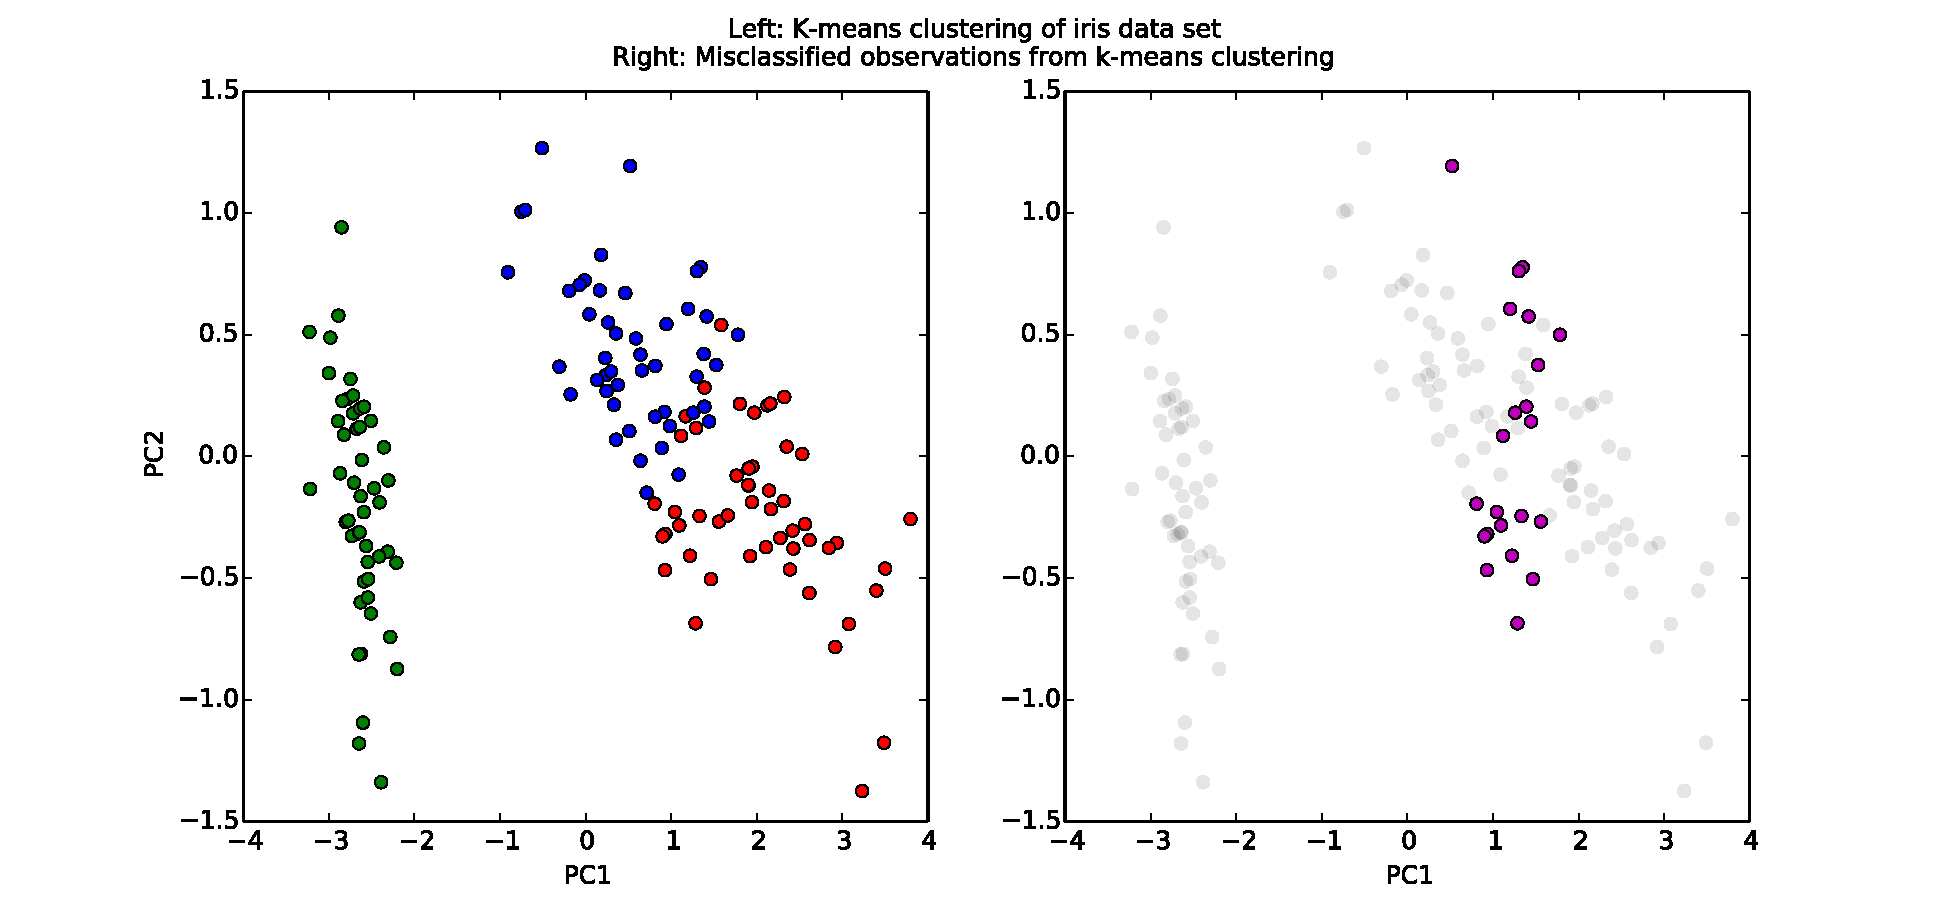
\includegraphics[width=0.9\textwidth]{./figures/hands-on9/fig-python-kmeans.pdf}}
  \caption{Results of applying k-means clustering to the iris data set, using the k-means algorithm impelmented in SciPy.\label{fig:pykmeans}}
\end{figure}


\medskip
\begin{assignment}
\small

Using the `naive' k-means clustering algorithm described in lecture, implement your own k-means clustering function in either Python or R.

Your function should take as input:
\begin{enumerate}
\item A distance matrix
\item an integer, $k$, giving the number of clusters
\item an integer, \verb|maxiter|, giving the maximum number of iterations of the algorithm to perform. NOTE: \verb|maxiter| is an upper limit; you might a choose other criteria for the algorithm to converge, but \verb|maxiter| will guarantee that it completes.
\end{enumerate}

Illustrate your function with application to a data set of your choice.


\end{assignment}

% \section{Minimum Spanning Tree in R}

% The package \texttt{ape} has an \texttt{mst()} function. Several others packages, including vegan also have minimum spanning tree functions. The |mst()| function takes a dissimilarity matrix as its input and returns a square adjacency matrix, $A$, where $A_{ij} = 1$ if $(i,j)$ is an edge in the MST or 0 otherwise.

% Here's an application of the MST function to the cities example you completed above.

% \begin{R}
% > library(ape) # install ape first if necessary
% > city.mst <- mst(as.dist(cities))
% > city.mst # see the adjacency matrix return by mst
% \end{R}

% If you want to create a nice looking plot you can use the  |mat2listw()| function in the package |spdep|. |mat2listw|  converts the adjacency matrix into a form that you can extract the neighbor information from:

% \begin{R}
% > library(spdep) # install spdep first if necessary
% > plot(city.location, type='n', xlab='PCoord1', ylab='PCoord2')
% > text(city.location, labels=names(cities))

% # note British spelling of 'neighbours'
% > plot(mat2listw(city.mst)$neighbours, city.location, add=T) 
% \end{R}





